\documentclass[tikz,border=10pt]{standalone}
\usepackage{amsmath}
\usepackage{tikz}
\usetikzlibrary{angles,quotes,calc}
\usetikzlibrary{arrows.meta,decorations.pathmorphing,backgrounds,positioning,fit,petri}
\usetikzlibrary{positioning}    % 相对位置宏包

\begin{document}

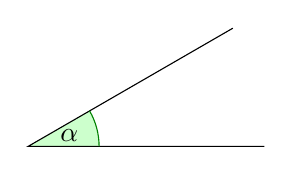
\begin{tikzpicture}[scale=3]
    % 绘制角度
    \coordinate(A)at(1,0);
    \coordinate(B)at(0,0);
    \coordinate(C)at(30:1cm);
    \draw(A)--(B)--(C)
    pic[draw=green!50!black,fill=green!20,angle radius=9mm,
    "$\alpha$"]{angle=A--B--C};
\end{tikzpicture}

\begin{tikzpicture}
    \path(0,2)node[shape=circle,draw]{}
    (0,1)node[shape=circle,draw]{}
    (0,0)node[shape=circle,draw]{}
    (1,1)node[shape=rectangle,draw]{}
    (-1,1)node[shape=rectangle,draw]{};
\end{tikzpicture}

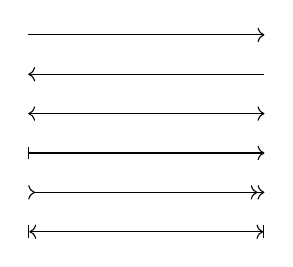
\begin{tikzpicture}
\draw[->] (0,2.5) -- (3,2.5);
\draw[<-] (0,2) -- (3,2);
\draw[<->] (0,1.5) -- (3,1.5);
\draw[|->] (0,1) -- (3,1);
\draw[>->>] (0,0.5) -- (3,0.5);
\draw[|<->|] (0,0) -- (3,0);
\end{tikzpicture}

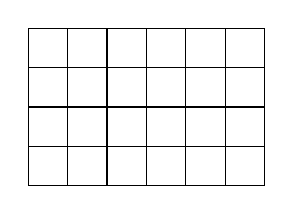
\begin{tikzpicture}
\draw[step=0.5] (0,0) grid (3,2);
\end{tikzpicture}

\begin{tikzpicture}
\draw[->] (0,0) -- (2,0);
\draw[->] (0,0) -- (0,2);
\node[below=4pt,left] at (0,0) {$O$};
\node[right] at (2,0) {$x$};
\node[above] at (0,2) {$y$};
\end{tikzpicture}

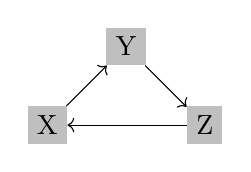
\begin{tikzpicture}
\node[fill=lightgray] (a) at (0,0) {X};
\node[fill=lightgray] (b) at (1,1) {Y};
\node[fill=lightgray] (c) at (2,0) {Z};
\draw[->] (a) -- (b);
\draw[->] (b) -- (c);
\draw[->] (c) -- (a);
\end{tikzpicture}

% 相对位置
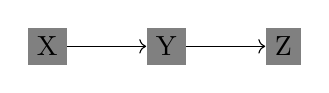
\begin{tikzpicture}
\node[fill=gray] (a) {X};
\node[fill=gray,right=1 of a] (b) {Y};
\node[fill=gray,right=1 of b] (c) {Z};
\draw[->] (a) -- (b);
\draw[->] (b) -- (c);
\end{tikzpicture}

\begin{tikzpicture}
\draw[->] (0,0) -- (4,0) node[right] {$x$};
\draw[->] (0,0) -- (0,3) node[above] {$y$};
\draw plot coordinates {(0,0) (1,2) (2,1) (4,3)};
\end{tikzpicture}

% 三维投影
\begin{tikzpicture}]
\draw[->] (-2,0,0) -- (2,0,0) node[right] {$x$};
\draw[->] (0,-1,0) -- (0,3,0) node[above] {$y$};
\draw[->] (0,0,-2) -- (0,0,2) node[below] {$z$};
\draw[color=red] plot[domain=0:2*pi] ({sin(\x r)},2,{cos(\x r)});
\draw[color=red] (0,0,0) -- (1,2,0) (0,0,0) -- (-1,2,0);
\end{tikzpicture}




\end{document}

